%! Author = chtompki
%! Date = 1/14/26
\documentclass[12pt]{amsart}
% Default margins are too wide all the way around. I reset them here
\setlength{\hoffset}{-.75in}
\setlength{\textwidth}{6.5in}
\setlength{\voffset}{-.5in}
\setlength{\textheight}{9.0in}
\usepackage{amsmath}
\usepackage{leftindex}
\usepackage{amssymb}
\usepackage{mathrsfs}
\usepackage{tikz}
\usepackage{amsthm}
\usepackage{enumitem}
\usepackage{setspace}
\usetikzlibrary{shadows,arrows,arrows.meta,shapes,positioning,calc,patterns}

\theoremstyle{definition}
\newtheorem{definition}{Definition}

\newenvironment{solution}
{\begin{proof}[Solution]}
{\end{proof}}

\tikzset{
    ell/.style={draw,ellipse,minimum height=6em,minimum width=10em,align=center},
    inner_ell/.style={draw,ellipse,minimum height=4em,minimum width=6em,align=center},
    ellthin/.style={draw,ellipse,minimum height=2em,minimum width=10em,align=center},
    line/.style={-,line width=0.5pt},
    dot/.style = {draw,fill,circle,inner sep=0pt,outer sep=0pt,minimum size=2pt},
    spot/.style = {draw,fill,circle,inner sep=0pt,outer sep=0pt,minimum size=0pt},
}

\title{Combinatorics\\Notes January 29, 2026}
%\author{Rob Tompkins}
\date{\today}

\begin{document}
    \maketitle
    \date{\today}
    \begin{onehalfspace}
        \section{Sterling Numbers. Con't}
        Let $f:M\rightarrow B$ be a function where $M$ is a set of marbles and $B$ is a set of boxes.
        Also let $m = |M|$ and $b = |B|$
        We concern ourselves with the following counts.
        \begin{enumerate}
            \item We want the count of the number of relations from $M$ to $B$:
                \begin{displaymath}
                    \text{count} = 2^{|M\times B|} = 2^{|M||B|} = 2^{mb}
                \end{displaymath}
            \item We want the count of the number of general functions from $M$ to $B$ which follows as:
                \begin{displaymath}
                    \text{count} = b^m
                \end{displaymath}
            \item With $m\leq b$ we want to count the number of one-to-one functions from $M$ to $B$ which follows
                  as:
                \begin{displaymath}
                    \text{count} = \leftindex_b P_m
                \end{displaymath}
            \item With $m \leq b$ we want to count the number of onto functions from $M$ to $B$, which follows as:
                \begin{eqnarray*}
                    \text{count} & = & b^m - \binom{b}{1}(b-1)^m + \binom{b}{2}(b-2)^m - \binom{b}{3}(b-3)^m + \cdots + (-1)^b\binom{b}{b}(b - b)^m \\
                                 & = & b! \cdot \frac{1}{b!} \sum_{k=0}^b (-1)^k\binom{b}{k}(b-k)^m = b!\mathcal{S}(m,b)
                \end{eqnarray*}
            \item With $m = b $ we want to count the number of bijections from $M$ to $B$. This follows as
                \begin{displaymath}
                    \text{count} = m! = b!
                \end{displaymath}
        \end{enumerate}
        Now we consider the diagram of the mapping $f:M\rightarrow b$
        \begin{figure}
            \centering
            \begin{tikzpicture}[>=Latex, every node/.style={font=\small}, set/.style={draw, thick}, inner/.style={draw, thick, pattern=north east lines, pattern color=gray!70}, map/.style={->, thick} ]
% Title
                \node[font=\large] at (5,4.2) {Linear Functions};
% --- Domain (left) ---
                \node at (2,3.2) {Domain};
% Outer oval M
                \draw[set] (2,1.5) ellipse (1.4 and 2.0);
                \node at (2,-0.8) {$M$};
% Inner shaded oval = kernel
                \draw[inner] (2,1.5) ellipse (0.65 and 1.35);
% Labels on left
                \node[align=left] at (0.1,1.6) {Kernel\\(Nullspace)};
                \node[align=left] at (0.4,2.45) {Pre-image};
% Sample points in domain
                \fill (1.85,2.1) circle (1.1pt) node[below left] {$m_1$};
                \fill (2.15,1.5) circle (1.1pt) node[below right] {$m_2$};
                \fill (1.95,0.9) circle (1.1pt) node[below left] {$m_3$};
% --- Codomain (right) ---
                \node at (8,3.2) {Codomain};
% Outer oval B
                \draw[set] (8,1.5) ellipse (1.4 and 2.0);
                \node at (8,-0.8) {$B$};
% Inner shaded oval = image/range
                \draw[inner] (8,1.5) ellipse (0.75 and 1.15);
% Labels on right
                \node[align=left] at (9.9,2.25) {$f(M)$\\Range};
                \node[align=left] at (9.65,1.55) {Image};
% Sample points in image
                \fill (7.9,1.95) circle (1.1pt) node[below left,label=270:$f(m_1)$] {};
                \fill (8.2,1.55) circle (1.1pt);
                \fill (7.85,1.10) circle (1.1pt);
% Label f over arrows
                \node[font=\normalsize] at (5,2.1) {$f$};
% --- Mapping arrows ---
                \draw[map] (1.85,2.1) .. controls (4.2,2.6) and (6.0,2.3) .. (7.9,1.95);
                \draw[map] (2.15,1.5) .. controls (4.0,1.8) and (6.2,1.9) .. (8.2,1.55);
                \draw[map] (1.95,0.9) .. controls (4.0,1.1) and (6.0,1.2) .. (7.85,1.10);
% Extra faint arrows to mimic the sketch
                \draw[->, thin, gray!60] (2.7,2.7) .. controls (4.8,2.4) and (6.8,2.7) .. (8.7,2.1);
                \draw[->, thin, gray!60] (2.7,0.4) .. controls (4.7,0.9) and (6.7,0.6) .. (8.7,1.0);
            \end{tikzpicture}
            \caption{Linear Functions}
        \end{figure}
    \end{onehalfspace}


\end{document}
